\documentclass{beamer}
\usepackage[slovene]{babel}
\usepackage{subcaption}
\newcommand{\ttitle}{Algoritmi za reševanje problema matričnih napolnitev}
\newcommand{\ttitleEn}{Algorithms for solving the matrix completion problem}
\newcommand{\tsubject}{\ttitle}
\newcommand{\tsubjectEn}{\ttitleEn}
\newcommand{\tauthor}{Matej Klančar}
\newcommand{\tkeywords}{matrične napolnitve, minimizacija ranga, rekonstrukcija slik, priporočilni sistemi}
\newcommand{\tkeywordsEn}{matrix completion, rank minimization, image reconstruction,
recommendation systems}
\newcommand{\nnorm}[1]{\lVert#1\rVert_*}
\newcommand{\fnorm}[1]{\lVert#1\rVert_F}
\newcommand{\norm}[1]{\lVert#1\rVert}
\newcommand{\CR}[1]{\begin{color}{red}#1\end{color}}
\newcommand{\CB}[1]{\begin{color}{blue}#1\end{color}}
\newcommand{\CG}[1]{\begin{color}{green}#1\end{color}}

\newcommand{\proj}{\mathcal{P}_\Omega}
\newcommand{\shrink}{\mathcal{D}}
%\newcommand{\tr}{\text{Tr}}
\newcommand{\numberthis}{\addtocounter{equation}{1}\tag{\theequation}}
\newcommand{\trOp}[2]{\langle #1, #2 \rangle}
\newcommand{\mapa}{Poglavja}

\DeclareMathOperator{\diag}{diag}
\DeclareMathOperator{\tr}{Tr}
\DeclareMathOperator*{\argmin}{arg\,min}

%Information to be included in the title page:
\title{Algoritmi za reševanje problema matričnih napolnitev}
\author[Matej Klančar]{Matej Klančar \\ \vspace{0.2cm} Mentor: doc.\ dr.\ Aljaž Zalar}
\usetheme{Madrid}
\date{2023}

\definecolor{colorTheme}{rgb}{0.19, 0.73, 0.56} % UBC Blue (primary)
\usecolortheme[named=colorTheme]{structure}
\setbeamercolor{alerted text}{fg=colorTheme}


\makeatletter
\setbeamertemplate{footline}
{
  \leavevmode%
  \hbox{%
  \begin{beamercolorbox}[wd=.25\paperwidth,ht=2.25ex,dp=1ex,center]{author in head/foot}%
    \usebeamerfont{author in head/foot}\insertshortauthor\expandafter\beamer@ifempty\expandafter{\beamer@shortinstitute}{}{~~(\insertshortinstitute)}
  \end{beamercolorbox}%
  \begin{beamercolorbox}[wd=.5\paperwidth,ht=2.25ex,dp=1ex,center]{title in head/foot}%
    \usebeamerfont{title in head/foot}\insertshorttitle
  \end{beamercolorbox}%
  \begin{beamercolorbox}[wd=.25\paperwidth,ht=2.25ex,dp=1ex,right]{date in head/foot}%
    \usebeamerfont{date in head/foot}\insertshortdate{}\hspace*{2em}
    \insertframenumber{} / \inserttotalframenumber\hspace*{2ex} 
  \end{beamercolorbox}}%
  \vskip0pt%
}
\makeatother

\AtBeginSection[]
{
    \begin{frame}
        \frametitle{Kazalo}
        \tableofcontents[currentsection]
    \end{frame}
}

\begin{document}
\selectlanguage{slovene}
\frame{\titlepage}
\section{Predstavitev problema}
\begin{frame}
  \frametitle{Predstavitev problema}
  \begin{itemize}
    \item Problem sprejme vhodno matriko M 
    \item Nekaterih elementov \alert{ne poznamo}
    \item Kako določiti manjkajoče elemente, da bo \alert{rang čim manjši}
  \end{itemize}
  \begin{align*}
  \argmin_{X} \hspace{0.3cm} &\text{rank}(X) \\
  \text{pod pogojem} \hspace{0.3cm} &\proj(X) = \proj(M)
  \end{align*}
\end{frame}

\begin{frame}
  \frametitle{Uporabe algoritmov}
  \begin{itemize}
    \item Priporočilni sistemi
    \item Rekonstrukcija signalov
    \item Računanje razdalj med napravami
    \item Rekonstrukcija slik
  \end{itemize}
\end{frame}

\section{Algoritmi}
\begin{frame}
  \frametitle{Algoritem NNM}
  \begin{itemize}
    \item Minimizira \alert{nuklearno normo} \[
            \nnorm{A} = \sum_{i = 1}^{n} \sigma_i(A)
          \]
    \item Rešuje problem semidefinitega programiranja
    \item Lahko rešujemo s primernimi orodji za reševanje takih problemov (npr. Sedumi)
  \end{itemize}
\end{frame}

\begin{frame}
  \frametitle{Algoritem SVT}
  \begin{itemize}
    \item Problem definira z \alert{Lagrangeovo funkcijo} \[
            \mathcal{L}(X, Y) = \tau \nnorm{X} + \frac{1}{2}\fnorm{X}^2 + \trOp{Y}{\proj(M-X)}
          \]
    \item Uporabimo t.i. \alert{Uzawa algoritem}, rešujemo iterativno
          \begin{align*}
            X^{(k)} & = \shrink_\tau(Y^{(k-1)}),                 \\
            Y^{(k)} & = Y^{(k-1)} + \delta_k \proj(M - X^{(k)}),
          \end{align*}
    \item \alert{Operator praga} $\shrink_\tau: \mathbb{R}^{n_1 \times n_2} \rightarrow \mathbb{R}^{n_1 \times n_2}$ je definiran kot
          \begin{align*}
            \shrink_\tau(A) & := U \shrink_\tau(\Sigma) V^T, \\ \shrink_\tau(\Sigma) &= \diag\big(\max(\sigma_1 - \tau, 0),
            \max(\sigma_2-\tau,0),\ldots,                    \\
                            & \hspace{1.5cm}
            \max(\sigma_{\min(n_1,n_2)}-\tau,0)\big)
          \end{align*}
    \item Uporabi idejo, da ima matrika majhnega ranga \alert{le nekaj velikih singularnih vrednosti}.
  \end{itemize}
\end{frame}

\begin{frame}
  \frametitle{Algoritem TNNM}
  \begin{itemize}
    \item Minimizira \alert{prirezano nuklearno normo} \[
            \norm{X}_r = \sum_{i = r + 1}^{\min(n_1, n_2)} \sigma_i(X)
          \]
    \item Uporabi $A_l, B_l$, sestavljeni iz \alert{lastnih vektorjev} $X$
    \item Uporablja iterativni algoritem \alert{ADMM}, definira pomožni matriki $W, Y$
          \begin{align*}
            X^{(k+1)} & = \shrink_\frac{1}{\beta}(W^{(k)} - \frac{1}{\beta} Y^{(k)}) \\
            W^{(k+1)} & = X^{(k+1)} + \frac{1}{\beta}(A_l^T B_l + Y^{(k)})           \\
            Y^{(k+1)} & = Y^{(k)} + \beta(X^{(k+1)}- W^{(k+1)})
          \end{align*}
  \end{itemize}
\end{frame}

\begin{frame}
  \frametitle{Algoritem ASD}
  \begin{itemize}
    \item Išče matriki $X, Y$ katerih \alert{produkt} bo enak rekonstrukciji
    \item Uporablja \alert{gradientni spust} nad funkcijo \[
            f(X, Y) = \frac{1}{2}\, \fnorm{\proj(M) - \proj(XY)}^2
          \]
    \item Z uporabo \alert{gradienta} in \alert{optimalnega koraka} izvaja premik
          \begin{align*}
            X^{(k+1)} = X^{(k)} - t_{x^{(k)}} \nabla f_{Y^{(k)}}(X^{(k)}) \\
            Y^{(k+1)} = Y^{(k)} - t_{y^{(k)}} \nabla f_{X^{(k+1)}}(Y^{(k)})
          \end{align*}
  \end{itemize}
\end{frame}

\begin{frame}
  \frametitle{Algoritem LMaFit}
  \begin{itemize}
    \item Uporablja \alert{Moore-Penrose inverz}
    \item Množenje rešuje po \alert{metodi najmanjših kvadratov}
          \begin{align*}
            X^{(k+1)} & = Z^{(k)}(Y^{(k)})^\dagger                           \\
            Y^{(k+1)} & = (X^{(k+1)})^\dagger Z^{(k)}                        \\
            Z^{(k+1)} & = X^{(k+1)}Y^{(k+1)} + \proj(M - X^{(k+1)}Y^{(k+1)})
          \end{align*}
  \end{itemize}
\end{frame}


\section{Rezultati}
\begin{frame}
  \frametitle{Vhodne slike}
  \begin{figure}
    \begin{subfigure}{0.325\linewidth}
      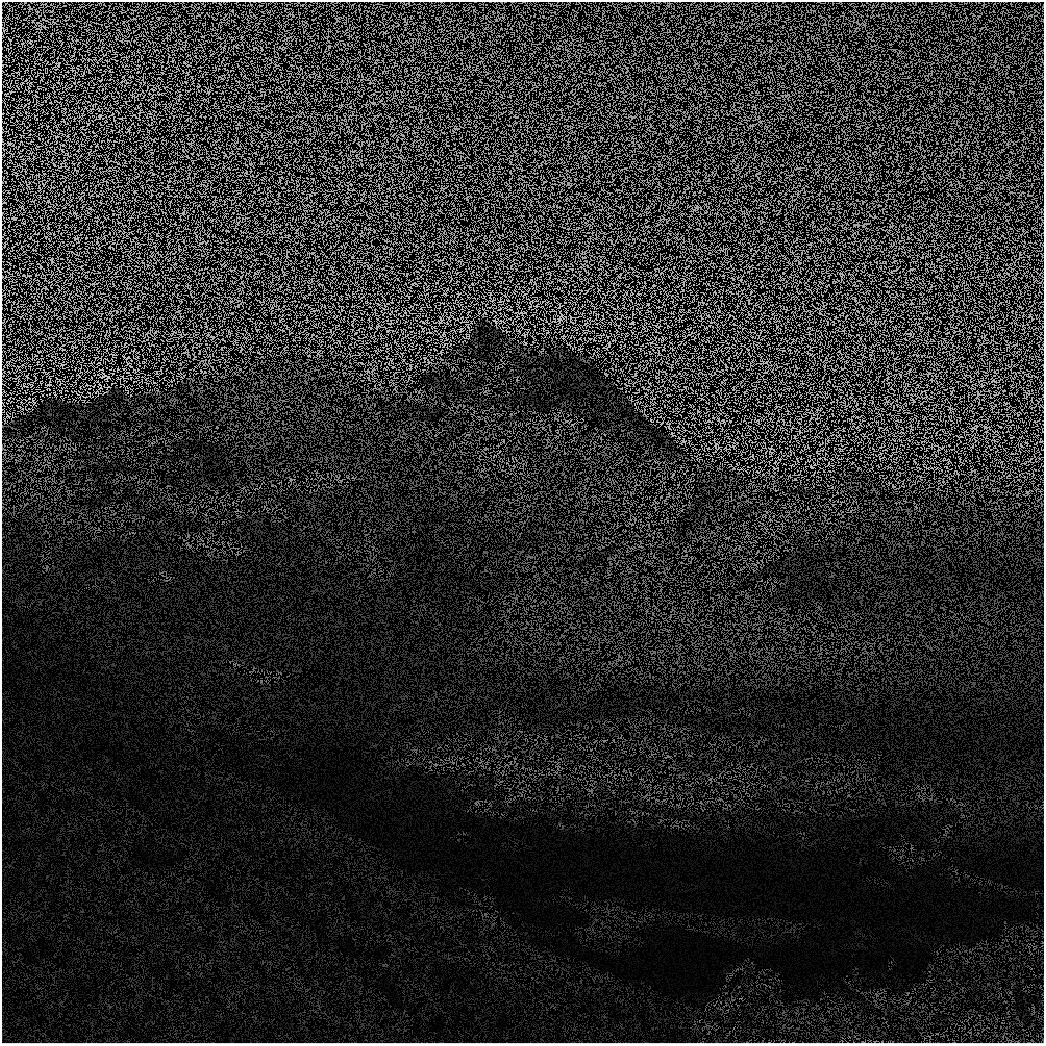
\includegraphics[width=\linewidth]{slike/vhod/slikaInput35.png}
      \caption{35\% znanih podatkov}
    \end{subfigure}
    \begin{subfigure}{0.325\linewidth}
      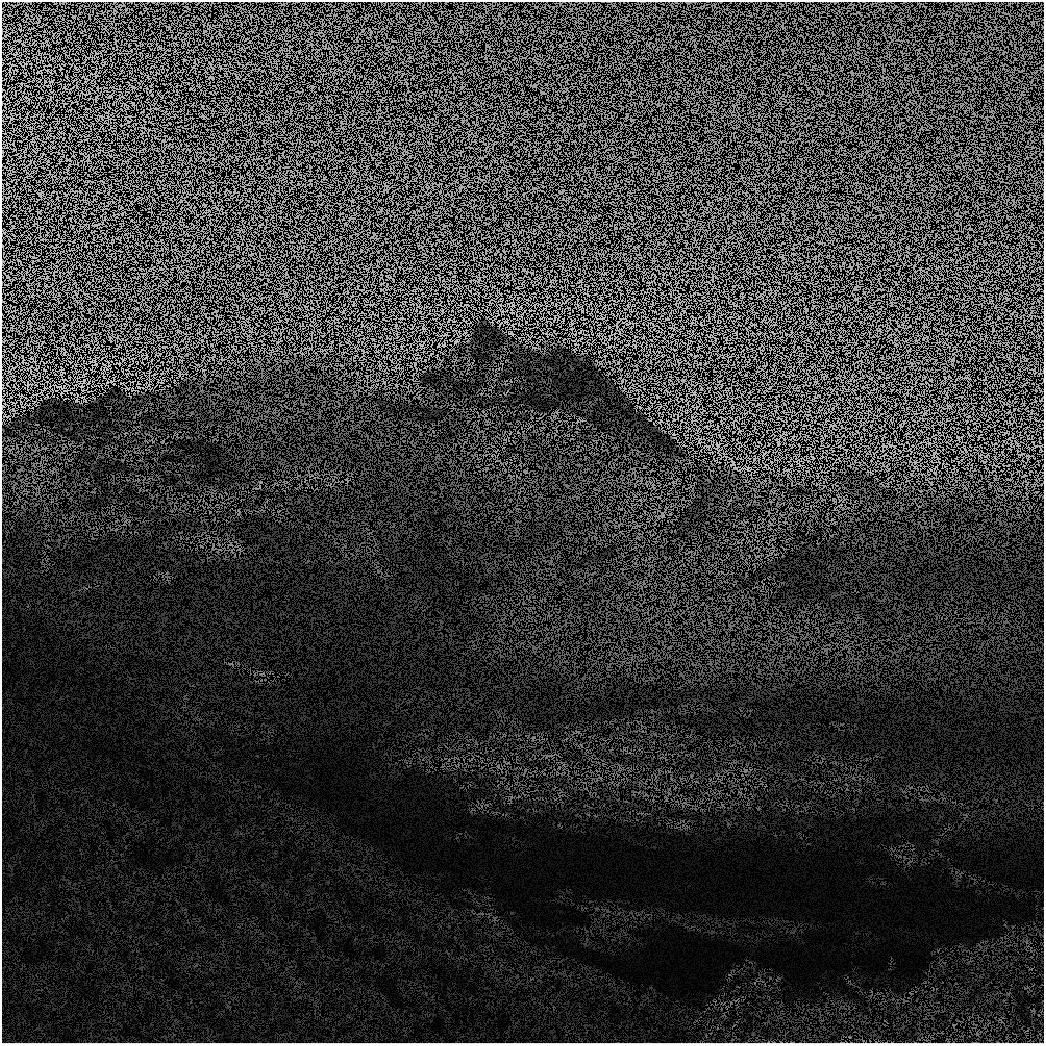
\includegraphics[width=\linewidth]{slike/vhod/slikaInput45.png}
      \caption{45\% znanih podatkov}
    \end{subfigure}
    \begin{subfigure}{0.325\linewidth}
      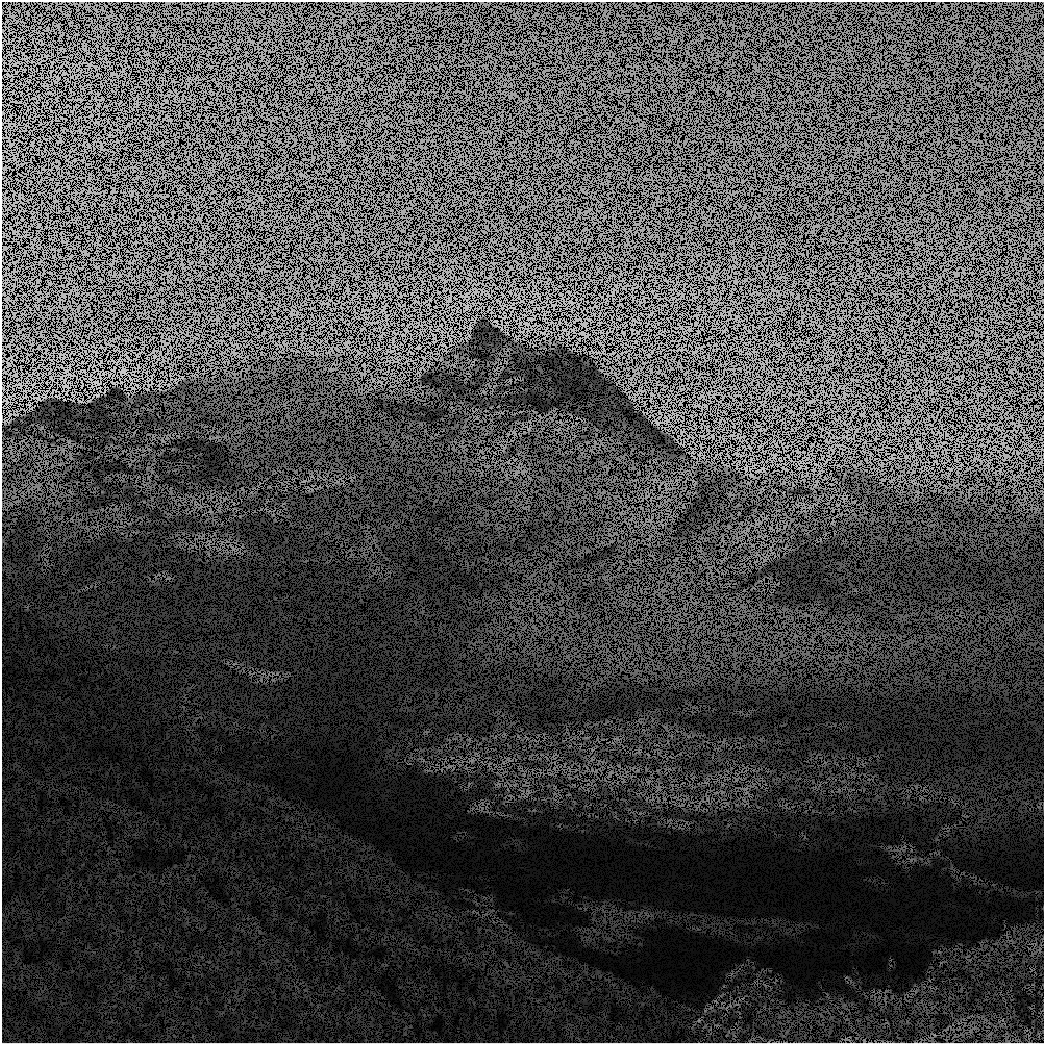
\includegraphics[width=\linewidth]{slike/vhod/slikaInput60.png}
      \caption{60\% znanih podatkov}
    \end{subfigure}
  \end{figure}
\end{frame}

\begin{frame}
  \frametitle{Rekonstrukcija z algoritmom SVT}
  \begin{figure}
    \begin{subfigure}{0.325\linewidth}
      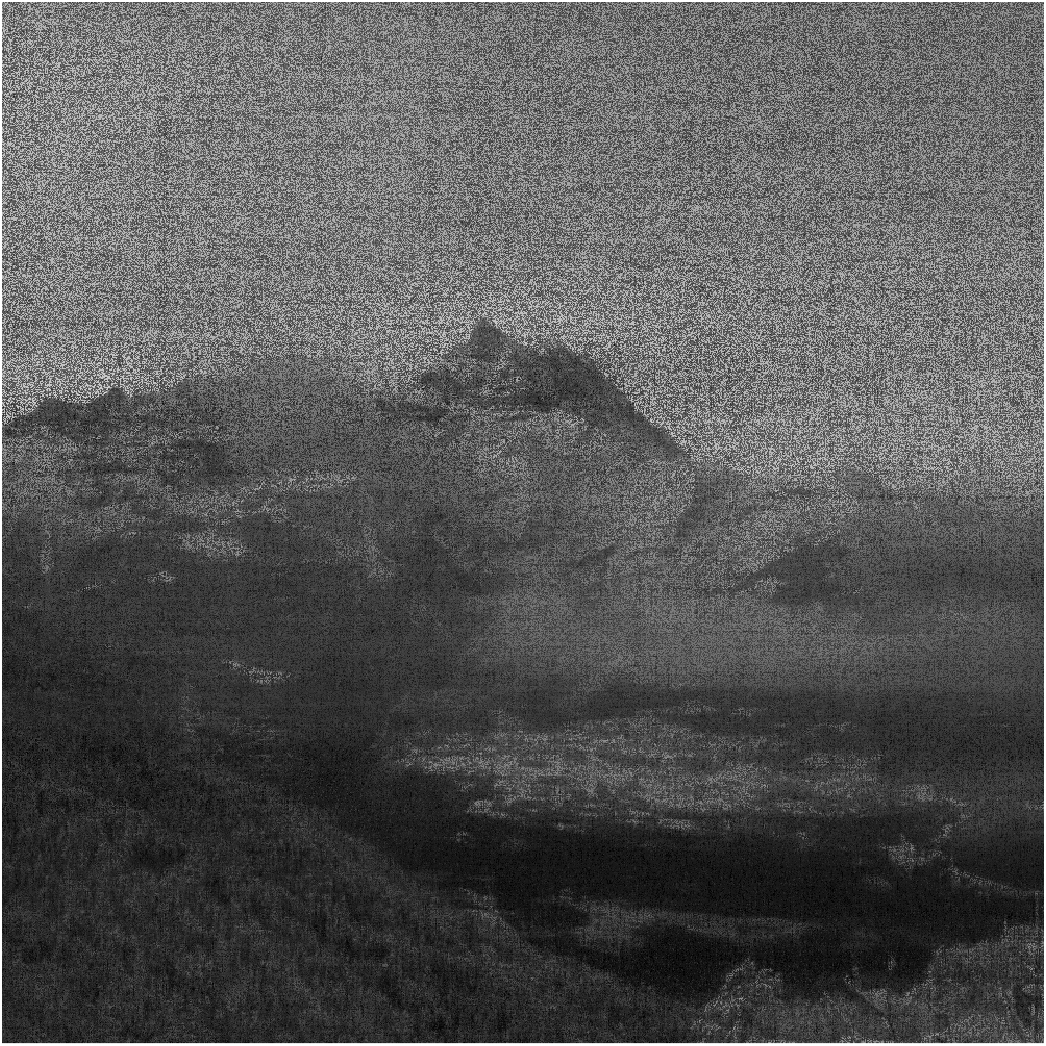
\includegraphics[width=\linewidth]{slike/gora/slikaRez35SVT.png}
      \caption{35\% znanih podatkov}
    \end{subfigure}
    \begin{subfigure}{0.325\linewidth}
      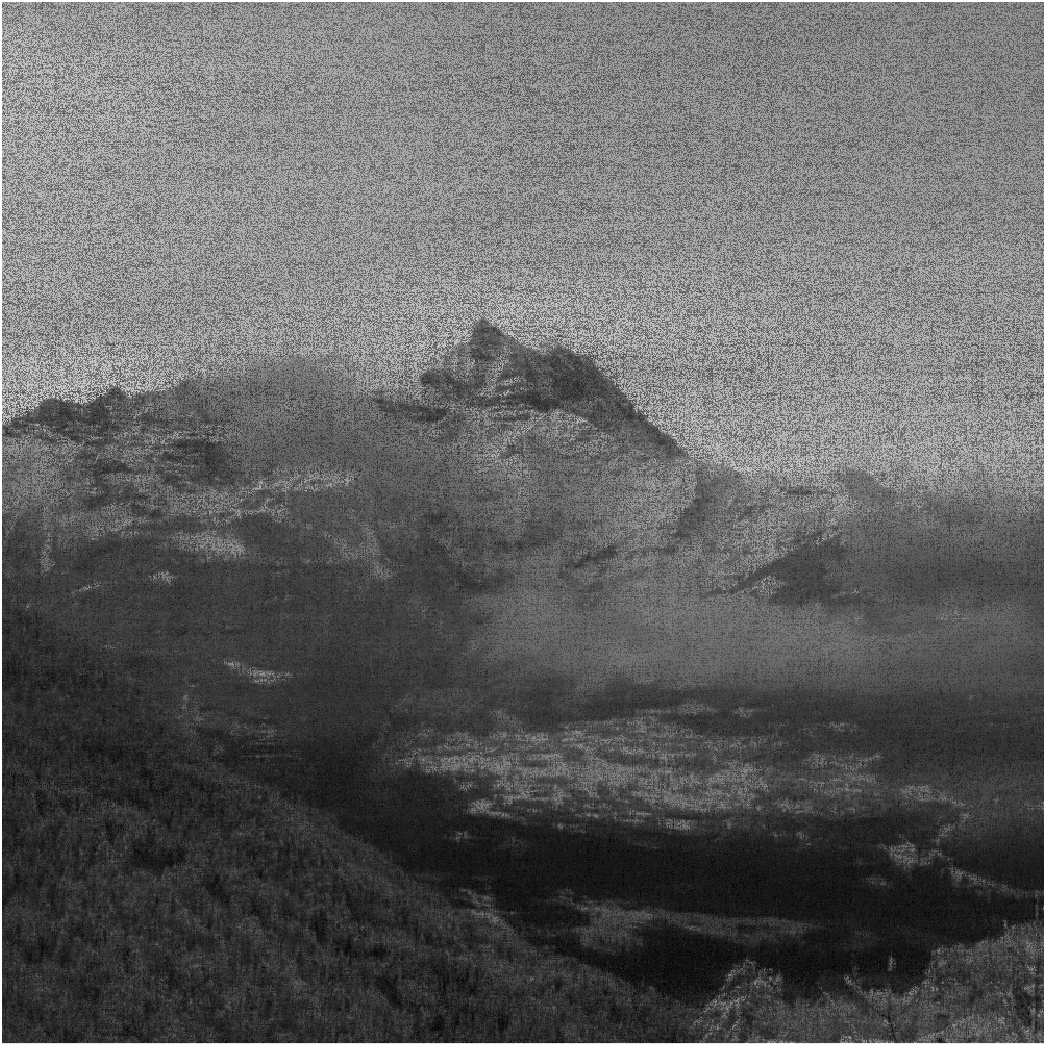
\includegraphics[width=\linewidth]{slike/gora/slikaRez45SVT.png}
      \caption{45\% znanih podatkov}
    \end{subfigure}
    \begin{subfigure}{0.325\linewidth}
      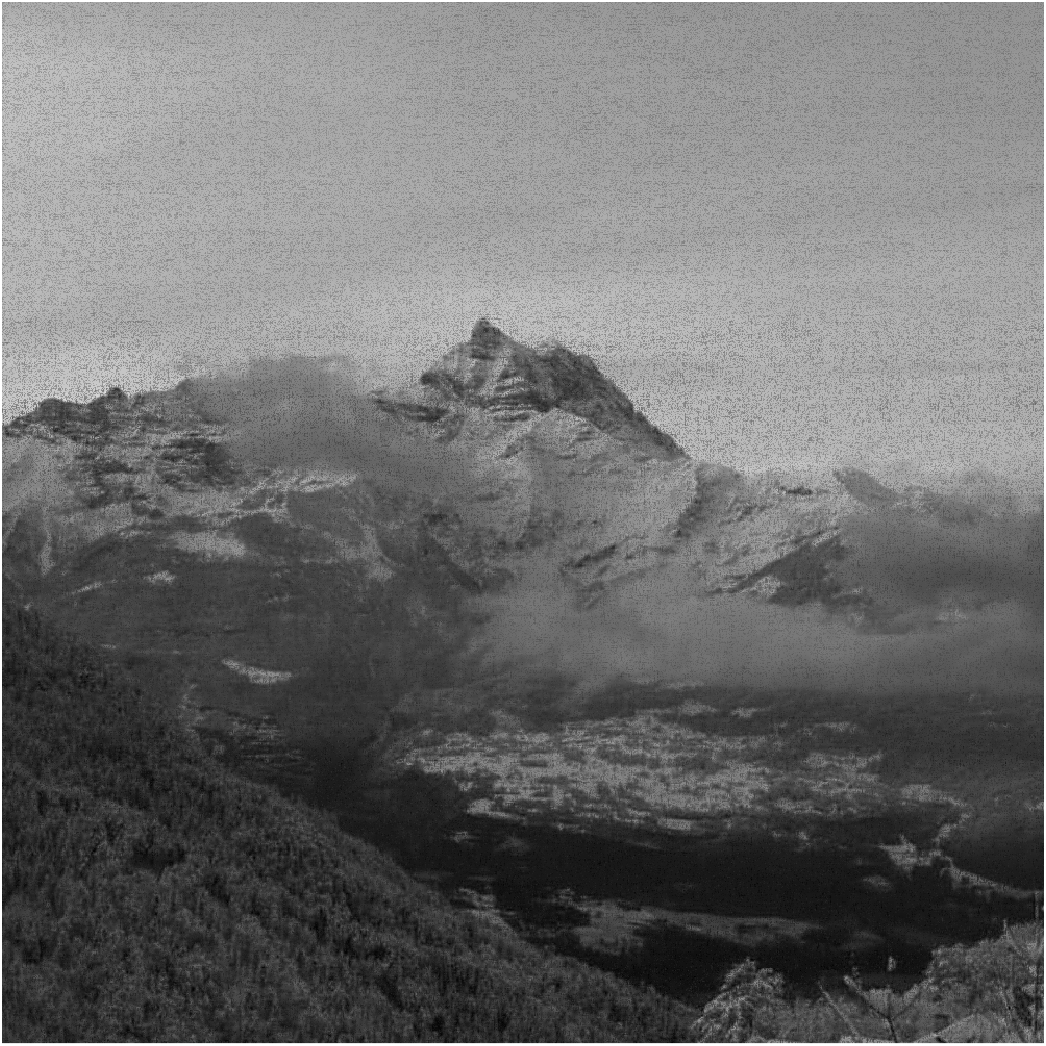
\includegraphics[width=\linewidth]{slike/gora/slikaRez60SVT.png}
      \caption{60\% znanih podatkov}
    \end{subfigure}
  \end{figure}
\end{frame}

\begin{frame}
  \frametitle{Rekonstrukcija z algoritmom TNNM}
  \begin{figure}
    \begin{subfigure}{0.325\linewidth}
      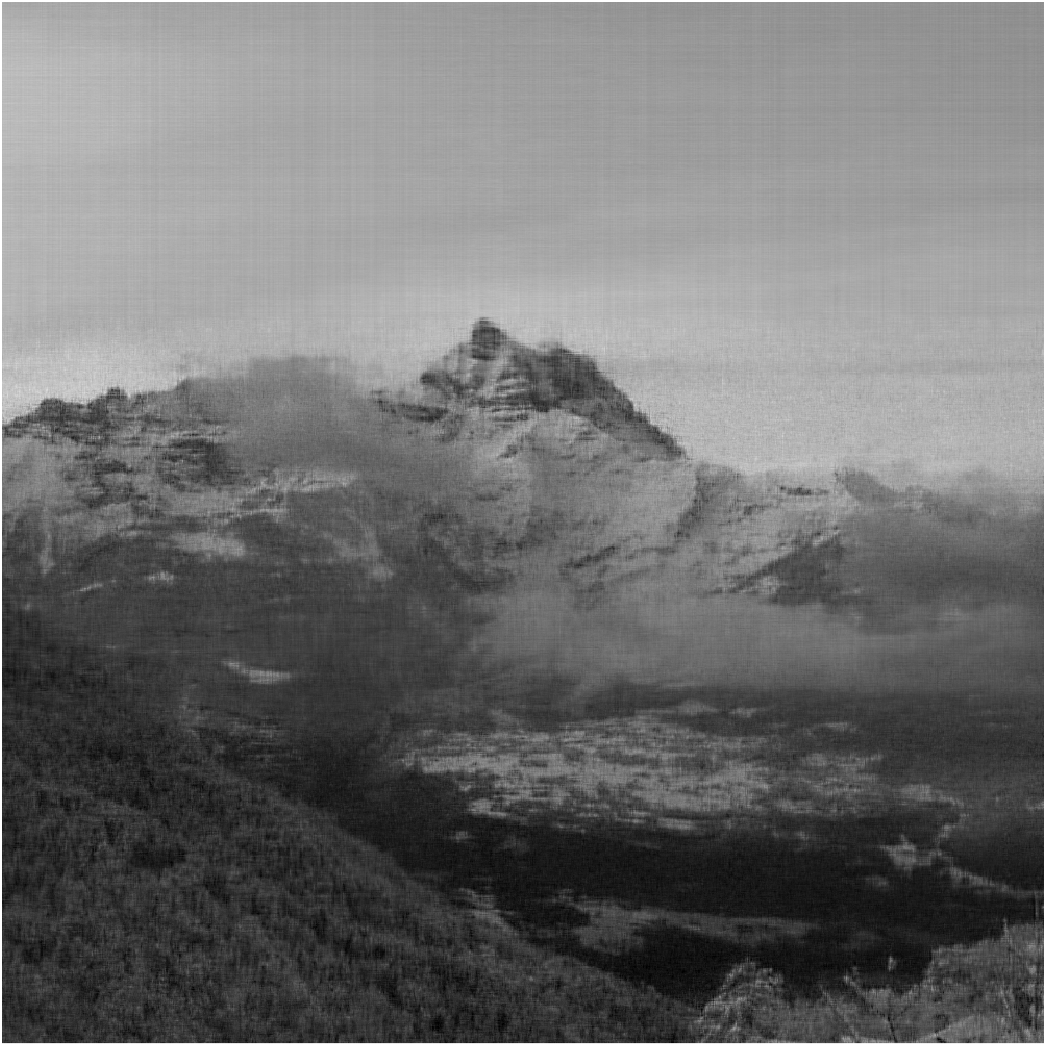
\includegraphics[width=\linewidth]{slike/gora/slikaRez35TNNM.png}
      \caption{35\% znanih podatkov}
    \end{subfigure}
    \begin{subfigure}{0.325\linewidth}
      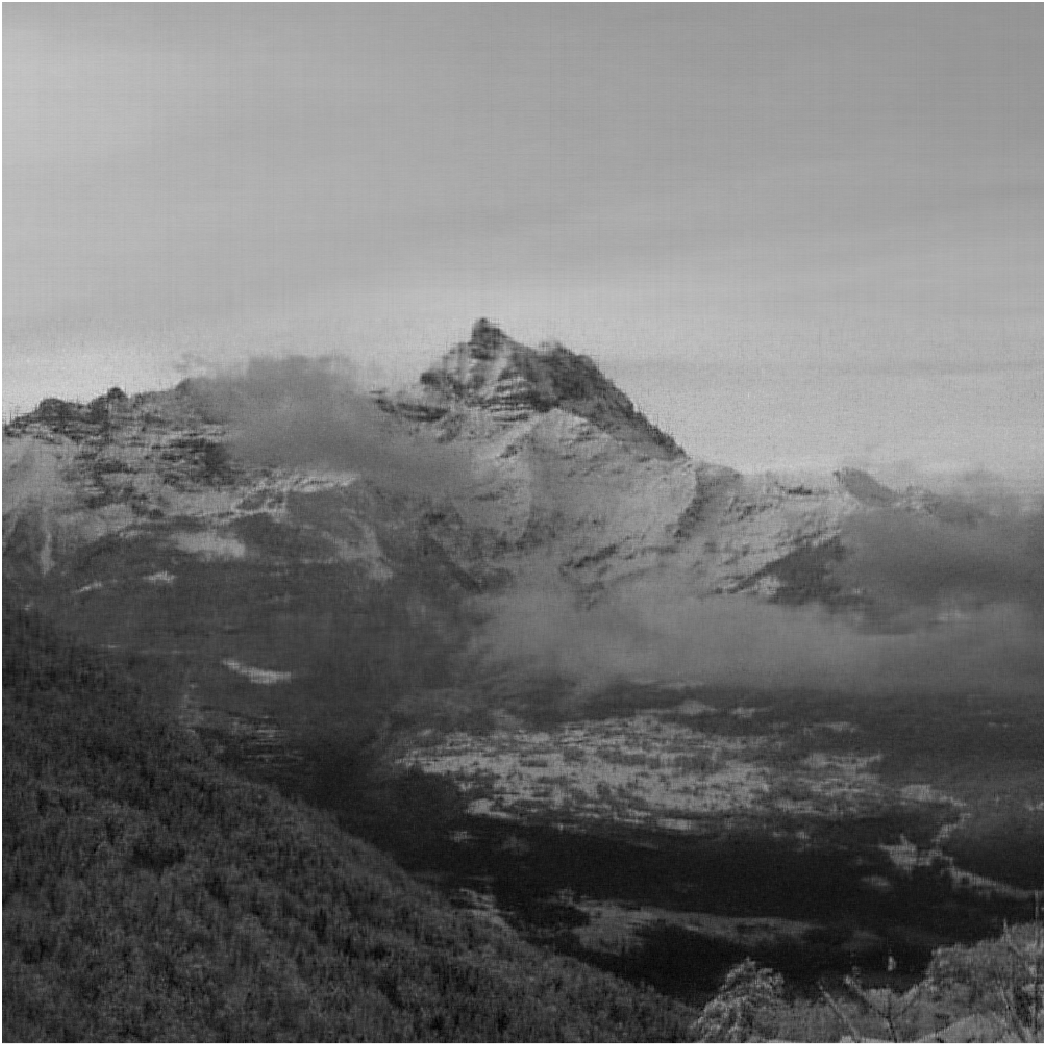
\includegraphics[width=\linewidth]{slike/gora/slikaRez45TNNM.png}
      \caption{45\% znanih podatkov}
    \end{subfigure}
    \begin{subfigure}{0.325\linewidth}
      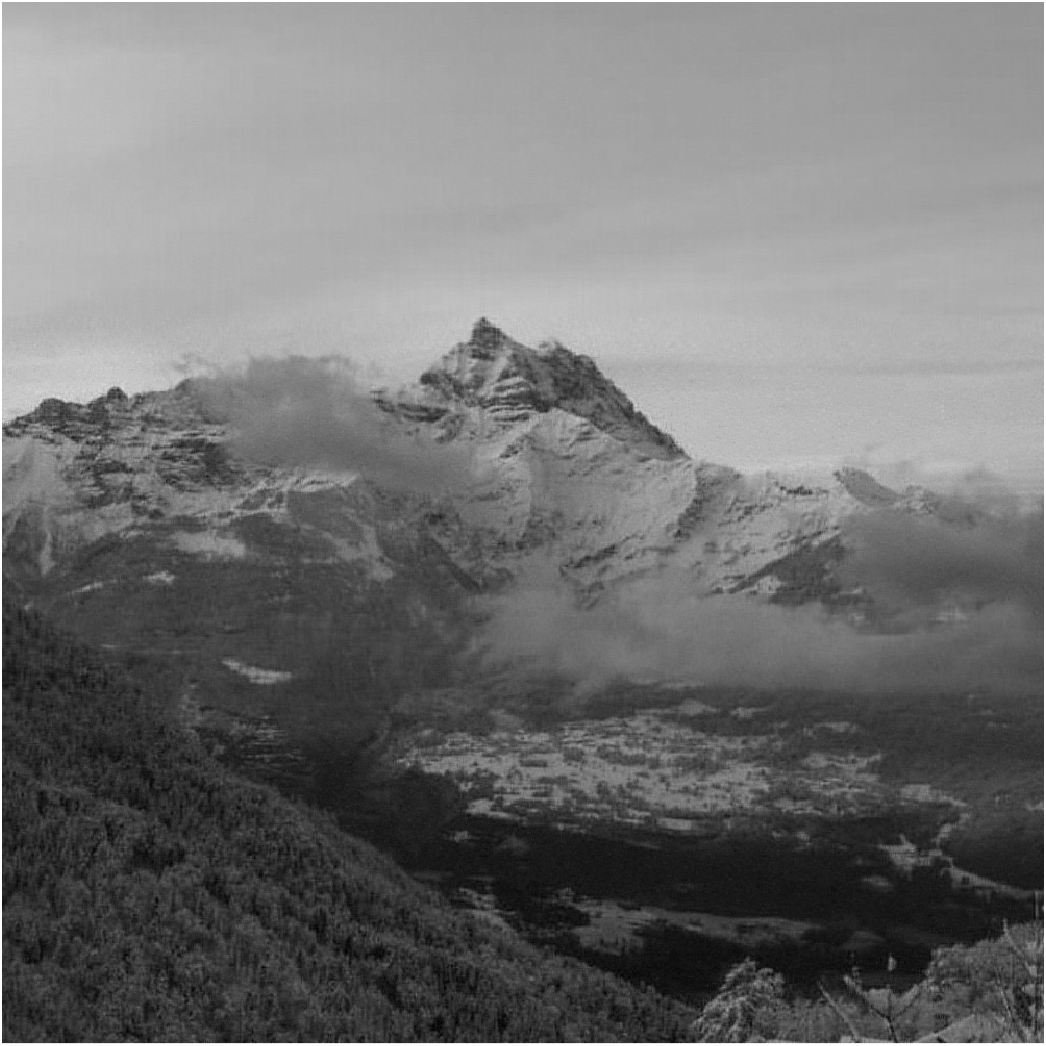
\includegraphics[width=\linewidth]{slike/gora/slikaRez60TNNM.png}
      \caption{60\% znanih podatkov}
    \end{subfigure}
  \end{figure}
\end{frame}

\begin{frame}
  \frametitle{Rekonstrukcija z algoritmom ASD}
  \begin{figure}
    \begin{subfigure}{0.49\linewidth}
      
\includegraphics[width=\linewidth]{slike/gora/slikaRez35ASD400.png}
      \caption{35\% znanih podatkov}
    \end{subfigure}
    \begin{subfigure}{0.49\linewidth}
      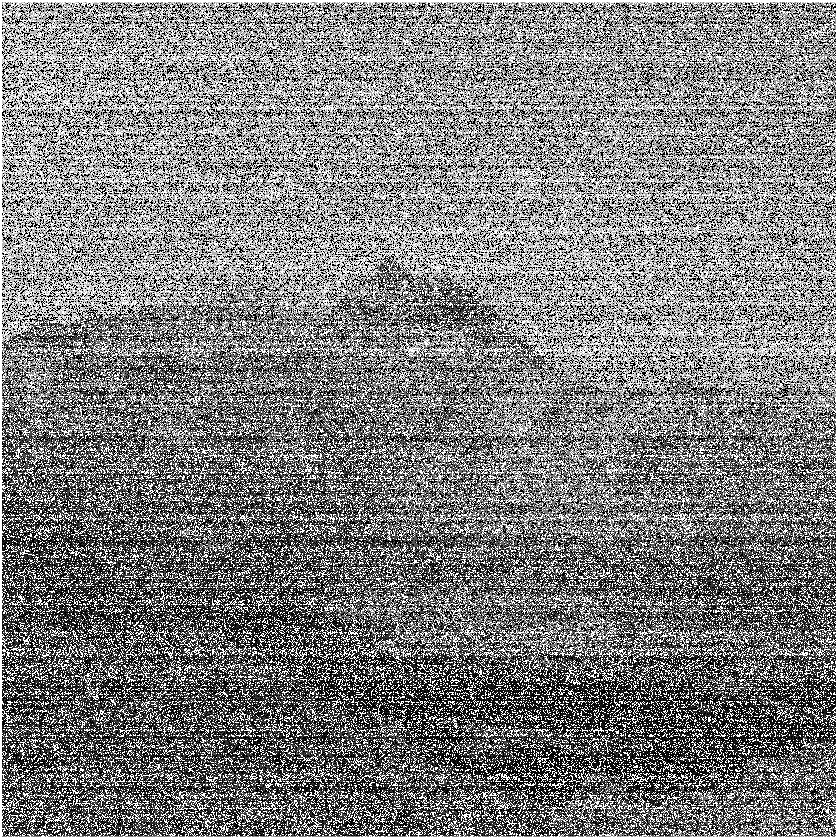
\includegraphics[width=\linewidth]{slike/gora/slikaRez45ASD600.png}
      \caption{45\% znanih podatkov}
    \end{subfigure}
  \end{figure}
\end{frame}

\begin{frame}
  \frametitle{Rekonstrukcija z algoritmom LMaFit}
  \begin{figure}
    \begin{subfigure}{0.325\linewidth}
      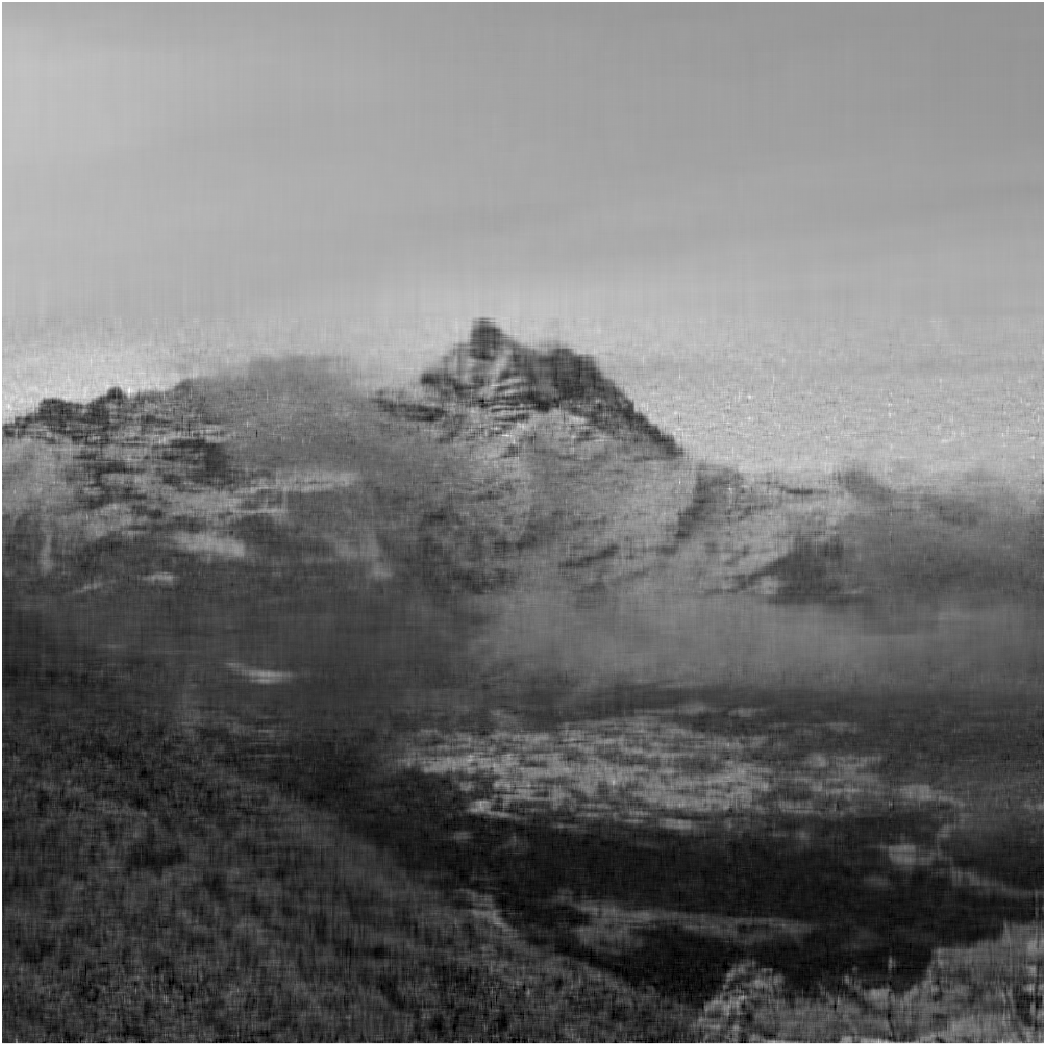
\includegraphics[width=\linewidth]{slike/gora/slikaRez35LmaFIT50.png}
      \caption{35\% znanih podatkov}
    \end{subfigure}
    \begin{subfigure}{0.325\linewidth}
      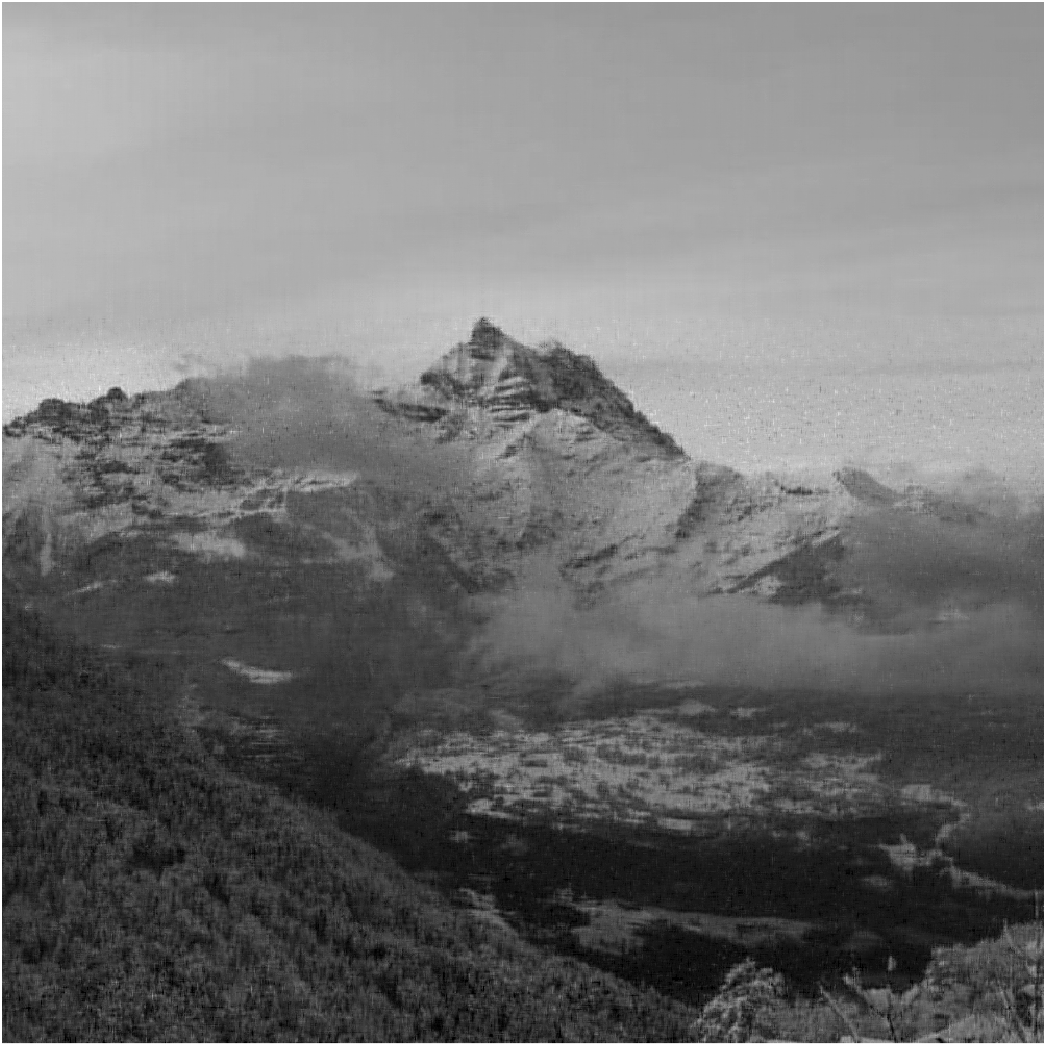
\includegraphics[width=\linewidth]{slike/gora/slikaRez45LmaFIT73.png}
      \caption{45\% znanih podatkov}
    \end{subfigure}
    \begin{subfigure}{0.325\linewidth}
      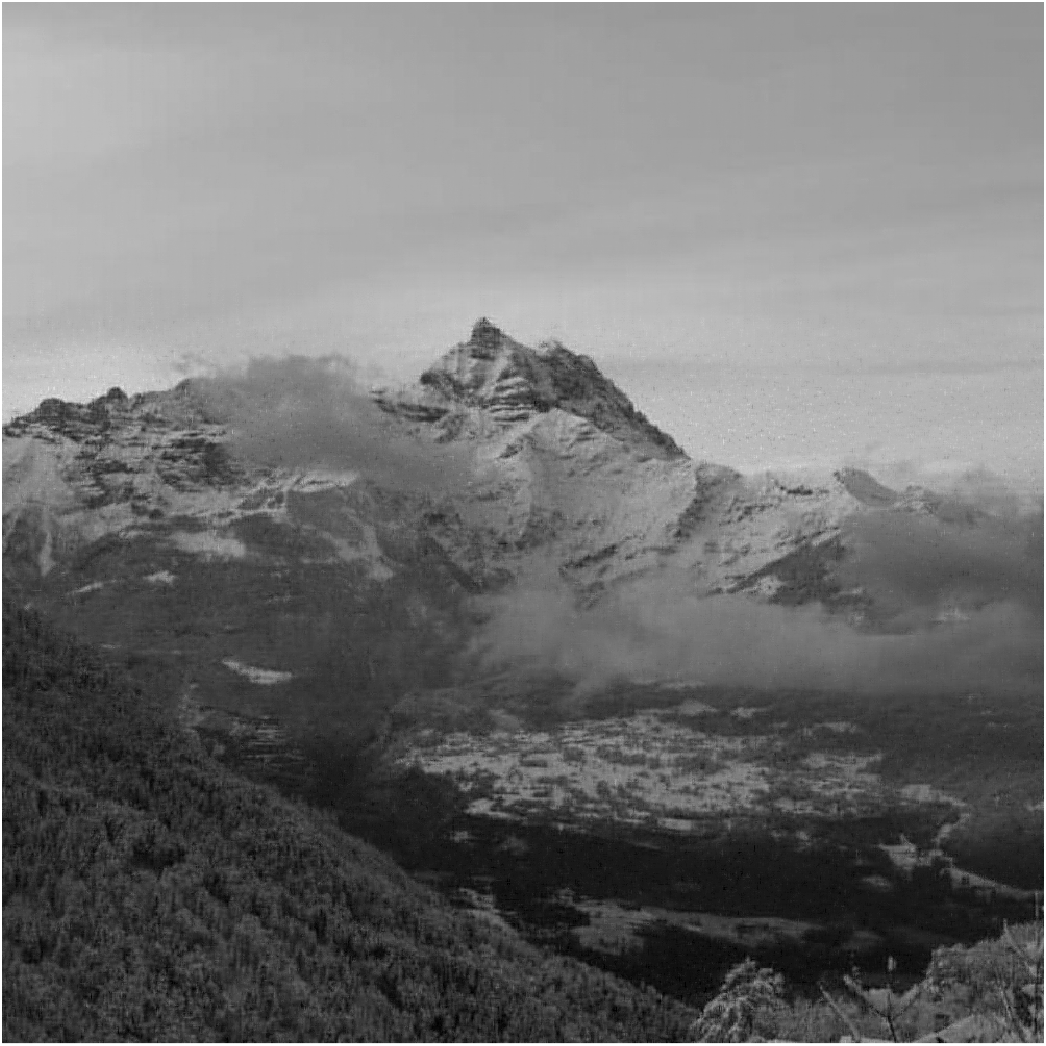
\includegraphics[width=\linewidth]{slike/gora/slikaRez60LmaFIT77.png}
      \caption{60\% znanih podatkov}
    \end{subfigure}
  \end{figure}
\end{frame}


\begin{frame}
  \frametitle{Napake algoritmov v Frobeniusovi normi}
  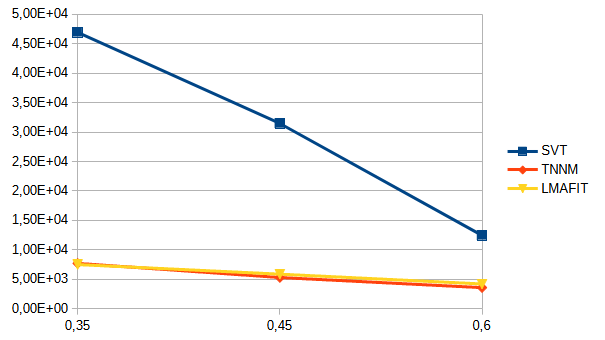
\includegraphics[width=\linewidth]{slike/gora/grafNapake.png}
\end{frame}

\begin{frame}
  \frametitle{Časi izvajanja algoritmov}
  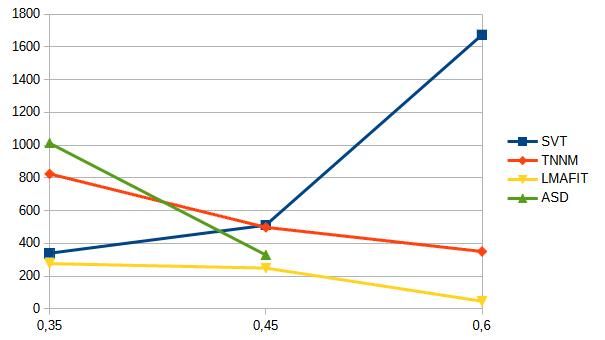
\includegraphics[width=\linewidth]{slike/gora/grafCas.png}
\end{frame}

\begin{frame}
  \frametitle{Vpliv kompleksnosti motiva pri algoritmu TNNM}
  \begin{figure}
    \begin{subfigure}{0.49\linewidth}
      
\includegraphics[width=\linewidth]{slike/kompleksnost/rez35TNNMprep.png}
      \caption{35\% znanih podatkov}
    \end{subfigure}
    \begin{subfigure}{0.49\linewidth}
      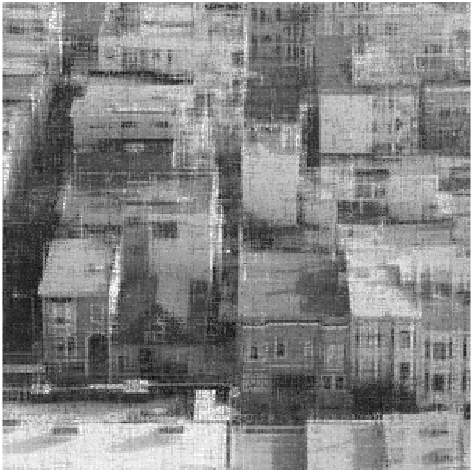
\includegraphics[width=\linewidth]{slike/kompleksnost/rez35TNNMkomp.png}
      \caption{35\% znanih podatkov}
    \end{subfigure}
  \end{figure}
\end{frame}

\begin{frame}
  \frametitle{Rekonstrukcija z reševanjem Laplaceovih diferencialnih enačb}
  \begin{figure}
    \begin{subfigure}{0.49\linewidth}
      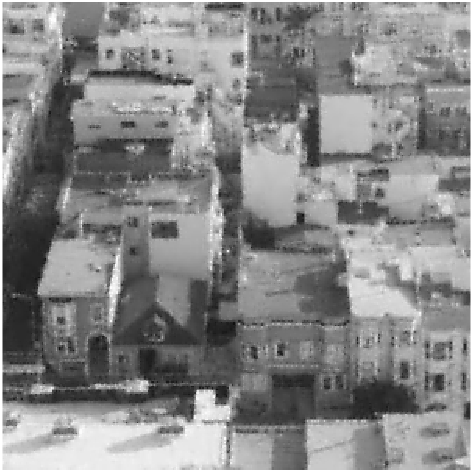
\includegraphics[width=\linewidth]{slike/laplac/rez35LapMesto.png}
      \caption{35\% znanih podatkov}
    \end{subfigure}
    \begin{subfigure}{0.49\linewidth}
      
\includegraphics[width=\linewidth]{slike/laplac/rez35LapDvobarvna.png}
      \caption{35\% znanih podatkov}
    \end{subfigure}
  \end{figure}
\end{frame}

\section{Zaključek}

\begin{frame}
  \frametitle{Ugotovitve}
  \begin{itemize}
    \item Algoritem LMaFit je najhitrejši
    \item Algoritem TNNM vrne najboljše rezultate
    \item Prednost algoritma SVT - ne potrebujemo informacije o rangu
    \item Algoritem NNM primeren za majhne matrike ($100 \times 100$)
    \item Ker se pri matričnih napolnitvah ne smemo zanašati na lokalno podobnost, obstajajo za rekonstrukcijo slik boljše metode
  \end{itemize}
\end{frame}


\begin{frame}
  \frametitle{Glavni prispevki}
  \begin{itemize}
    \item Implementacija algoritmov
    \item Primerjava delovanja algoritmov 
    \item Analiza vplivov parametrov
    \item Interpretacija rezultatov prek matematičnega ozadja
  \end{itemize}
\end{frame}

\end{document}